\section*{Summary}

This project is devoted to the development of an embedded application which controls an industrial lift that transports heavy loads between two floors.\medskip

From the get-go, the main goal of the project was to develop an optimized and efficient application, with proper configuration of the clocks, the interrupts, the IO and a few extra peripherals. \medskip

As per the lab sessions, the Keil uVision IDE was used to program the code and manage the files. In addition, STM32CubeMX was also used to configure the internal clocks.\medskip

The first step to tackling the problem was to carefully read the requirements and to create a diagram containing the desired workflow.\medskip

Once clarified, the peripherals were then configured one-by-one to accommodate for the different requirements. A modular approach was decided upon so as to simplify and organize the implementation. 

\section{Flowchart}
There are two main variables which control the functioning of the infinite loop, \textbf{\textit{buttonPressFlag}} and \textbf{\textit{timer5sEndFlag}}, both of them are initialized to false (these are Boolean variables). The first one is set to true when the interrupt attached to the button, EXTI0, is triggered. The second one, as its name states, is set when the 5 second timer (TIM3), overflows. Both are reset in the infinite loop.

\begin{figure}[H]
    \centering
    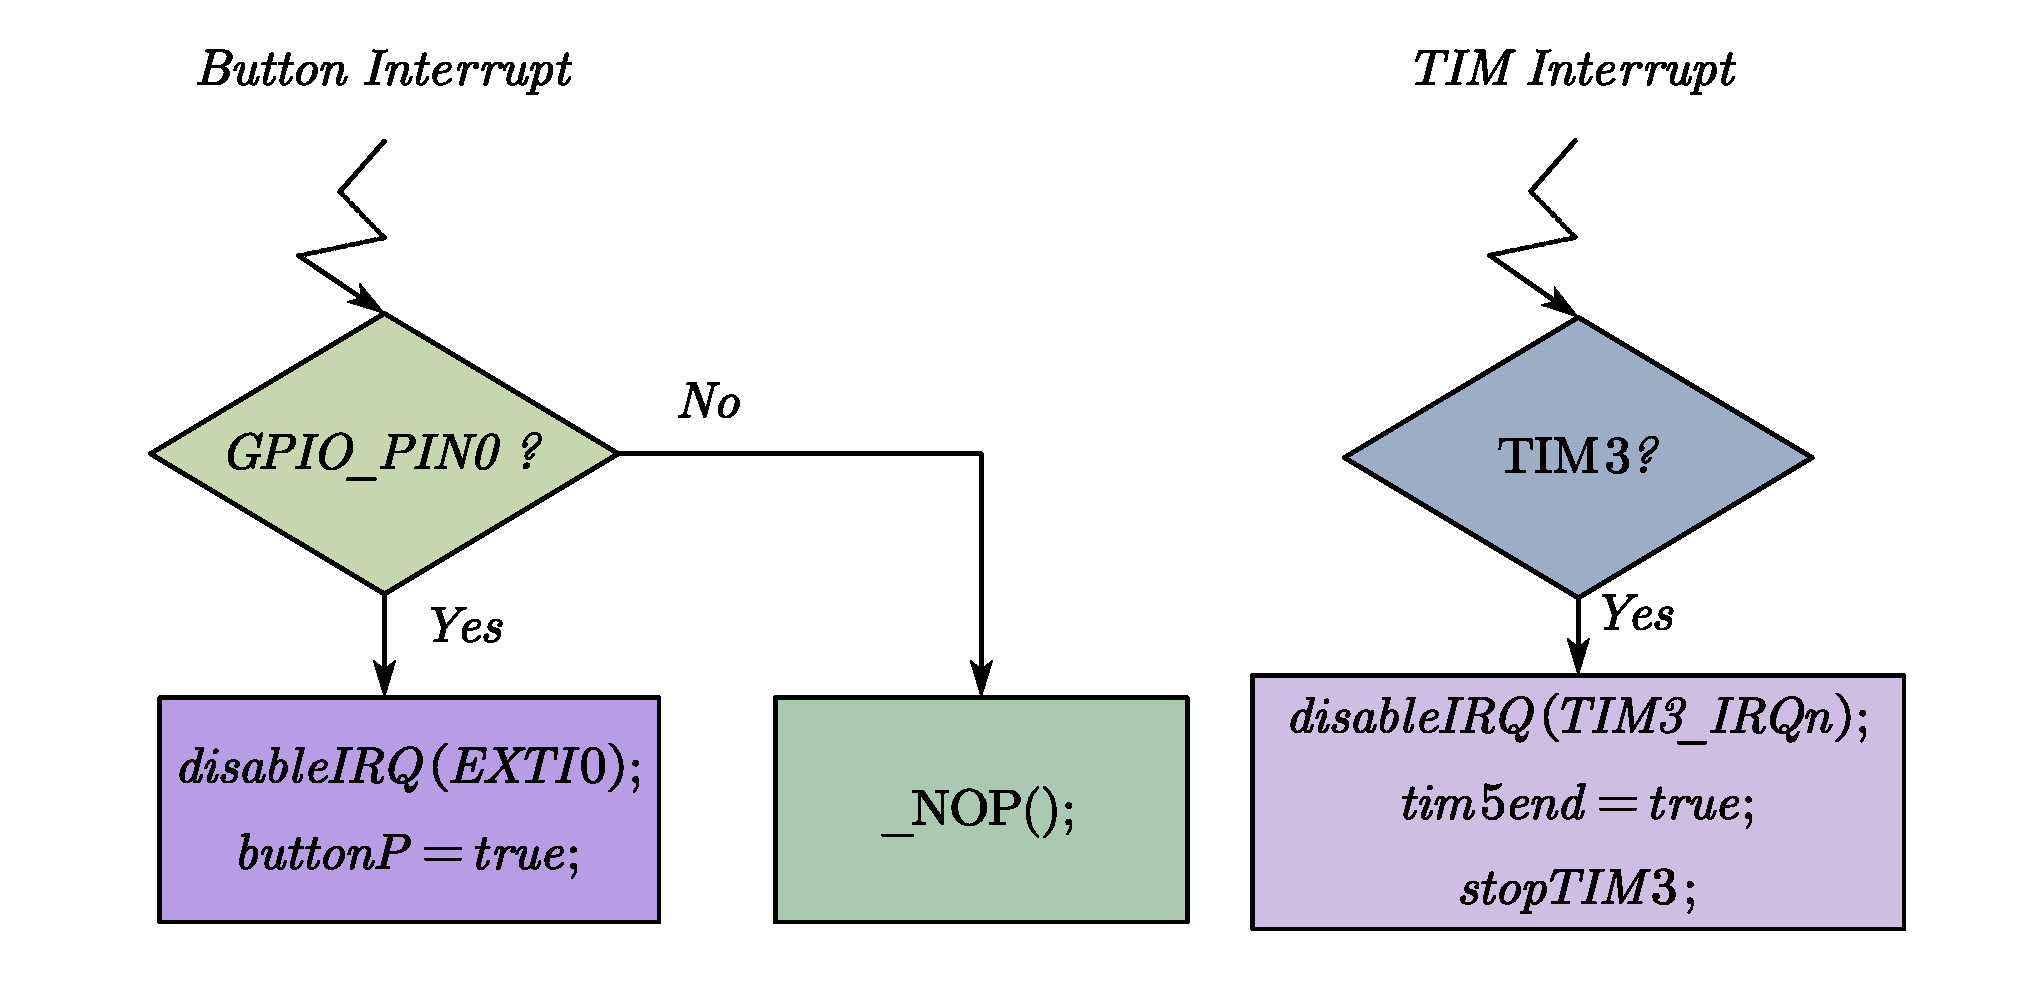
\includegraphics[width=0.7\textwidth]{Graphics/AXGLYPH_PDF/TIM_ISR.pdf}
    \caption{Interrupts workflow}
    \label{fig:Interrupts_workflow}
\end{figure}

After the main initialization, in the main loop, the system checks whether the \textbf{\textit{ButtonPressFlag}} is set. If it is, first the flag is reset, and, depending on the current floor, the next action is to go up or down. Inside the functions \textit{liftUp()} and \textit{liftDown()}, first the doors are closed, then the direction of the movement is decided, the LEDs are set to blink in the correct pattern, and finally, the timer 3 is started. The direction of the lift is sent via the UART.
\medskip

Then, the \textbf{\textit{timer5EndFlag}} is polled. If its value is $true$, the function \textit{liftStop()} is called, which re-enables both the EXTI0 IRQ and the TIM3 IRQ, turns off orange and red LEDs, sets the current floor depending on the lift direction, and opens the doors. In addition, it also sends the current floor through the UART.

\begin{figure}[H]
    \centering
    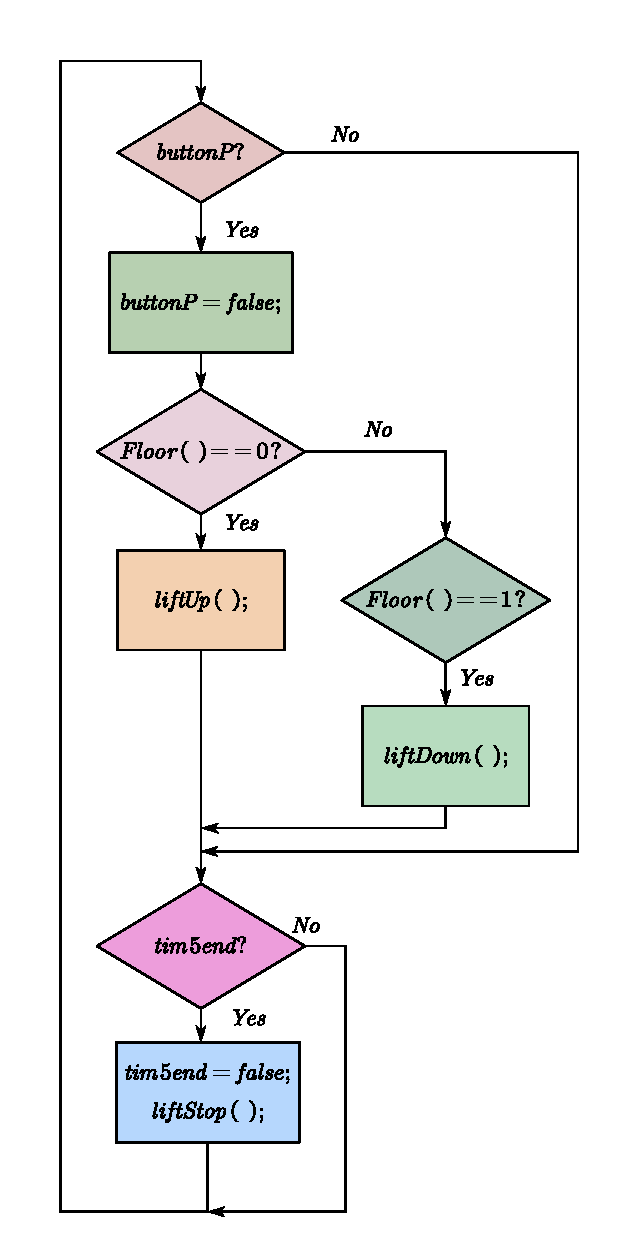
\includegraphics[scale=0.5]{Graphics/AXGLYPH_PDF/FLOWCHART.pdf}
    \caption{Flow chart describing the operation of the main loop}
    \label{fig:while_loop}
\end{figure}

\subsection{Files and functions}

Instead of defining all the required functions in just one file, we created the \textit{main.c} file following the simple structure explained in previous sections, and a main function file, \textit{lift.c}, which calls different functions from other sub-files to perform the wanted actions.

\medskip

This is a brief explanation of each file:

\begin{itemize}
    \item \textbf{\textit{button.c} :} Initializes the button hardware as well as its interrupt.
    \item \textbf{\textit{doors.c} :} Initializes the servomotors hardware and the functions to control the angle of their shaft. As two main positions are desired (open/close), each of them has its independent function.
    \item \textbf{\textit{led.c} :} Initializes the LEDs hardware and PWM, includes a function to set the PWM duty cycle, turns off the red and orange LEDs, and sets all LEDs to its initial state. The blue and green ones are controlled by an independent function which turns them on/off depending on the state of the lift (on a floor or moving).
    \item \textbf{\textit{lift.c} :} This file is the main nexus. It calls the different functions of the sub-files to control the main actions of the lift, such as initialization, move up/down, stop, retrieve the current floor, etc.
    \item \textbf{\textit{motor.c} :} Initializes the stepper motor GPIO.
    \item \textbf{\textit{timer.c} :} Configures the timers used in this application, TIM1, TIM3 and TIM4.
    \item \textbf{\textit{uart.c} :} Manages the initialization of the UART communication.
\end{itemize}

All of these files are strictly necessary for the proper operation of our application. As it can be seen on the project, inside "Core/Src" there are more files: \textit{stm32f4xx\_hal\_msp.c}, which is necessary for the MSP initialization and de-initialization; \textit{stm32f4xx\_it.c}, which is indispensable for interrupts; \textit{system\_stm32f4xx.c}, that initializes the system; \textit{stm32f4xx\_hal\_uart.c}, essential for UART module operation (this file would be, initially, inside the HAL drivers folder but since from the point of view of the CubeMX this peripheral is unused, it does not generate this file. To solve this problem, we got this file from another project in which we had configured the UART from CubeMX and included it in our source code folder.) 

Inside "Core/Inc", apart from the header files of the named files, we also find \textit{stm32f4xx\_hal\_conf.h}, which defines which peripherals are active.

\begin{cBox}
If "Generate code" is clicked in CubeMX, in the file \textit{stm32f4xx\_hal\_conf.h}, the UART and Timers peripherals will \textbf{NOT} be enabled. To solve this, it is necessary to uncomment lines 65 and 66 of said file.

\end{cBox}

\medskip

The set of functions shown in the sub-files were organized in the following way. (We also developed more functions, but these are the main ones used in \textit{lift.c}).

\begin{figure}[H]
    \centering
    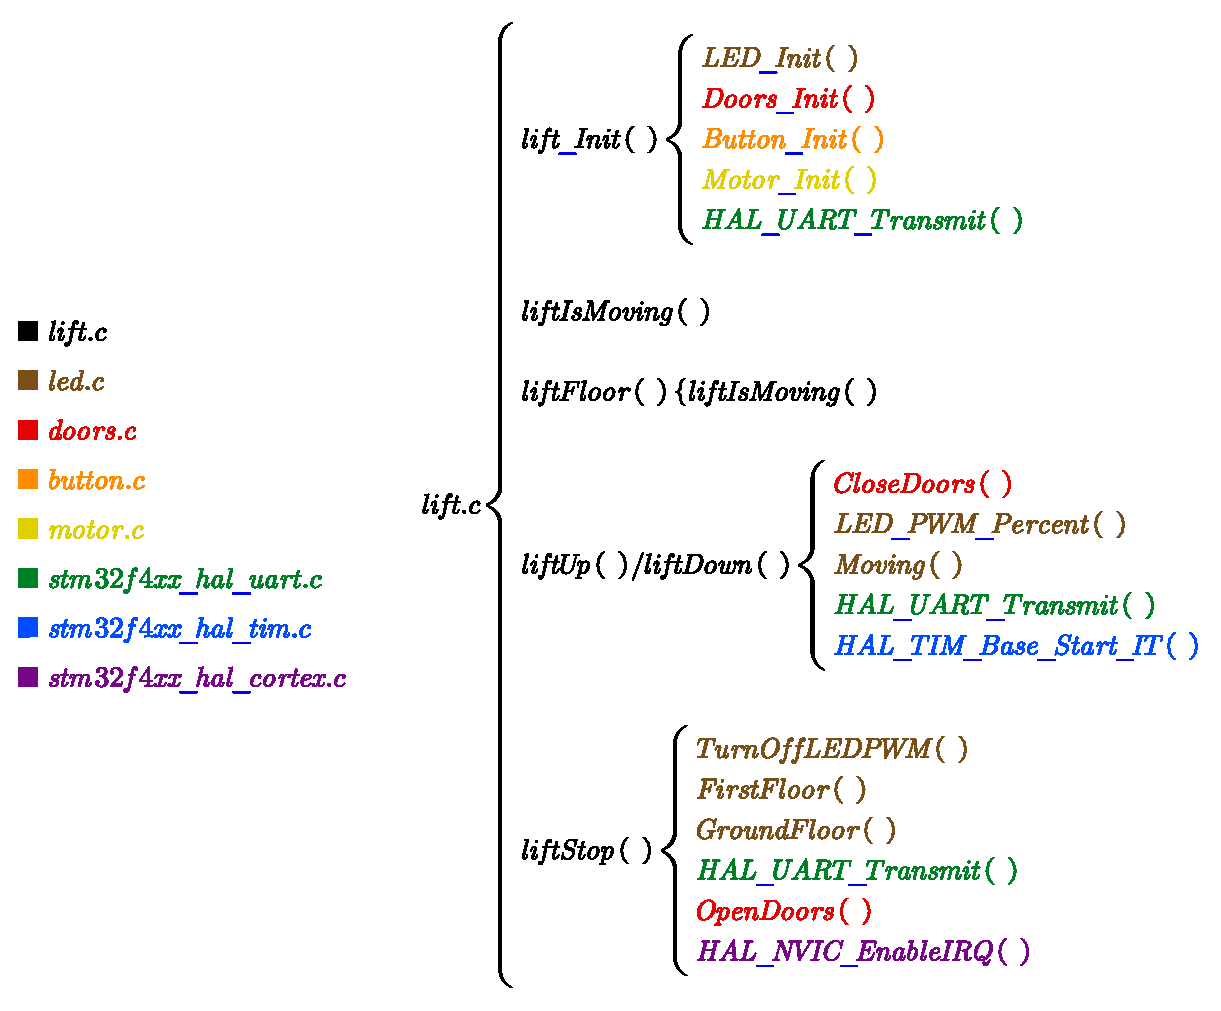
\includegraphics[width=0.60\textwidth]{Graphics/AXGLYPH_PDF/TREE.pdf}
    \caption{File dependency tree} 
    \label{fig:File_management}
\end{figure}

\section{Clocks and peripherals configuration}

As in this project, more peripherals than the strictly necessary ones were used, we will firstly introduce the essential ones and then, the rest.

\subsection{Minimum configuration}

As the problem states, the input consists of a button, and the outputs are 4 LEDs, which are already on the STM32F407 Discovery board. \medskip

The button, as stated before, must produce an interrupt, due to this, the EXTI0 interrupt was configured to trigger following the press of the blue button. \medskip

The green LED and the blue one were connected to simple push-pull outputs. No external resistors were required for this application. As the frequency did not matter in this case, we configured it as low.\medskip

The other two LEDs, orange and red, were configured to be controlled by Pulse Width Modulation. Since both share the same period, 1 second, they were configured with the same timer, in this case, TIM4. On the actual pin configuration, these pins had to be configured as alternate function push-pull. The internal resistor and speed parameters were configured mimicking the previously defined LED configuration. These LEDs in particular needed an extra configuration step: on the enumerated type variable \textit{GPIO\_InitStruct, Alternate}, the timer that controls them had to be configured as well for them to work as expected. \medskip

In order to control the duty cycle of the LEDs, a special function was developed, which takes the LED pin as an input, as well as the desired duty cycle, and both computes and writes the required pulse value to the CCRx register.

\inputCcode{Code/LED_PWM_Percent.c}

\medskip

Regarding the internal clock, the configuration was practically the same as the one that we used for the different lab sessions, namely, setting the internal clock to 100 MHz, and the APB1 and APB2 clocks to 1/2 of that.\medskip

As we needed a 1s period PWM, these values for the prescaler and counter were used:

\begin{equation*}
        \hspace{0.35cm} \mathrm{TIM4 \;} (\mathrm{T} = 1\;\mathrm{s)} \rightarrow \left\{ \begin{aligned}
	        \mathrm{TIM4 \; CLK} &= \,\, \dfrac{50\;\mathrm{MHz}}{\mathrm{Presc}} \, = \,\, \dfrac{50\;\mathrm{MHz}}{5000} = 10\;\mathrm{kHz}\\[\bigskipamount]
	        \,\, \mathrm{Counter \; period} &= \left( \left( \mathrm{TIM4 \; CLK} \right) \cdot \mathrm{T} -\,\,1 \right) = 999\\
        \end{aligned} \right. \\[\bigskipamount]
\end{equation*} 

In order to count the 5 seconds, which correspond to the time that it takes for the lift to move, timer 3 was chosen.  

\begin{equation*}
    \hspace{0.35cm} \mathrm{TIM3 \;} (\mathrm{T} = 5\;\mathrm{s)} \rightarrow \left\{ \begin{aligned}
	        \mathrm{TIM3 \; CLK} &= \,\, \dfrac{50\;\mathrm{MHz}}{\mathrm{Presc}} \, = \,\, \dfrac{50\;\mathrm{MHz}}{50000} = 1\;\mathrm{kHz}\\[\bigskipamount]
	        \,\, \mathrm{Counter \; period} &= \left( \left( \mathrm{TIM3 \; CLK} \right) \cdot \mathrm{T} -\,\,1 \right) = 4999\\
    \end{aligned} \right. \\[\bigskipamount]
\end{equation*}

\newpage

\subsection{Extra peripherals}

Two servomotors and one stepper motor were also used to increase the complexity of the project. For communications, the aforementioned UART peripheral was used in order to send information about the current action/set of actions. \medskip

To operate the servomotors, a PWM signal was used, the minimum pulse width of which was 0.75 ms; the maximum 2.25 ms. Its frequency, as per the manufacturer datasheet~\autocite{Parallax} was set to 50 Hz. The timer chosen to generate this signal was TIM1. Since we had two servomotors, we used two of the timer's channels (Connected to pins PE9 and PE11.)\medskip 

In order to control the angle, a special function was developed which takes the servomotor pin as an input, as well as the desired angle, and both computes and writes the required PWM pulse value to the corresponding CCRx register. 

\inputCcode{Code/Servo_PWM_Angle.c}

The timer 1 configuration was configured as follows:

\begin{equation*}
    \hspace{0.35cm} \mathrm{TIM4 \;} (\mathrm{T} = 1\;\mathrm{s)} \rightarrow \left\{ \begin{aligned}
	   \mathrm{TIM4 \; CLK} &= \,\, \dfrac{50\;\mathrm{MHz}}{\mathrm{Presc}} \, = \,\, \dfrac{50\;\mathrm{MHz}}{5000} = 10\;\mathrm{kHz}\\[\bigskipamount]
	    \,\, \mathrm{Counter \; period} &= \left( \left( \mathrm{TIM4 \; CLK} \right) \cdot \mathrm{T} -\,\,1 \right) = 999\\
   \end{aligned} \right. \\[\bigskipamount]
\end{equation*}

For the stepper motor to work properly, it needed a Look-Up Table and 1 ms wait between step changes. As the SysTick timer generates an interrupt every 1 ms, we decided to take advantage of this predefined interruption, reducing the necessary number of extra timers. Depending on the direction of the motor, the index of the LUT gets increased or decreased in each call. This can be observed in the following code:

\inputCcode{Code/SysTick_Handler.c}

\medskip

The UART was configured in order to have an asynchronous communication, with a baud rate of 9600, which is a common value for this type of communications.\medskip

In order to make the microcontroller transmit information, we used the HAL function designed for this purpose. This is an example of its usage:

\inputCcode{Code/uart.c}

\medskip

Summing up, all the pins configurations can be found below:

\begin{itemize}
    \item Blue Pushbutton 
        \begin{itemize}
            \item \textbf{PA0:} GPIO\_EXTI0, no pull-up no pull-down. 
        \end{itemize}
    
    \item UART Communication
        \begin{itemize}
            \item \textbf{PA2, PA3:} USART2\_TX, USART2\_RX.
        \end{itemize}
    
    \item Stepper Motor
        \begin{itemize}
            \item \textbf{PB12, PB13, PB14, PB15:} GPIO\_Output, Push-Pull, no internal resistor, output speed low.
        \end{itemize}
    
    \item Servomotor
        \begin{itemize}
            \item \textbf{PE9:} TIM1\_CH1.
            \item \textbf{PE11:} TIM1\_CH2.
        \end{itemize}
        
    \item Floor Number LEDs
        \begin{itemize}
            \item \textbf{PD12 (Green Led), PD15 (Blue Led)}: GPIO\_Output, Push-Pull, no internal resistor, output speed low.
        \end{itemize}
        
    \item State LEDs
        \begin{itemize}
            \item \textbf{PD13 (Orange Led):} TIM4\_CH2.
            \item \textbf{PD14 (Red Led):} TIM4\_CH3.
        \end{itemize}
        
\end{itemize}

\section{Conclusion}

This project is the culmination of months of work on this subject. We have applied the knowledge obtained in class to the best of out abilities, with gratifying results. In the end, everything worked as expected, even though we spent more time than we would like to admit debugging the code. This was due to the ordeal of configuring the peripherals without the aid of CubeMX, the "vanishing" of documents like \textit{stm32f4xx\_hal\_uart.c} and the need to uncomment a couple of lines from other files, which took a while to figure out. \medskip

That being said, we are really happy with how the project turned out in the end. In \href{https://github.com/anacalo24/MicroProject}{\textbf{this link}} you can find the project's GitHub repository, and, in \href{https://www.youtube.com/watch?v=KtsXlKJ0ibM}{\textbf{this one}} the video of the presentation and operation of the project. We hope that you like it!
